\chapter{Prototype}

\section{Le premier prototype (2018-2019)}

\noindent
Dans le cadre du projet d’année de la première année du Master ingénieur civil en informatique, un prototype capable de surveiller l’infrastructure de CERHIS a été réalisé. Ce dispositif s’inspirait sur d’autres prototypes plus anciens créés par des étudiants de l’école polytechnique de Bruxelles. L’architecture du dispositif produit l’année dernière est présentée sur la figure \ref{fig:archi_prev}.

~

\begin{figure}[ht!]
  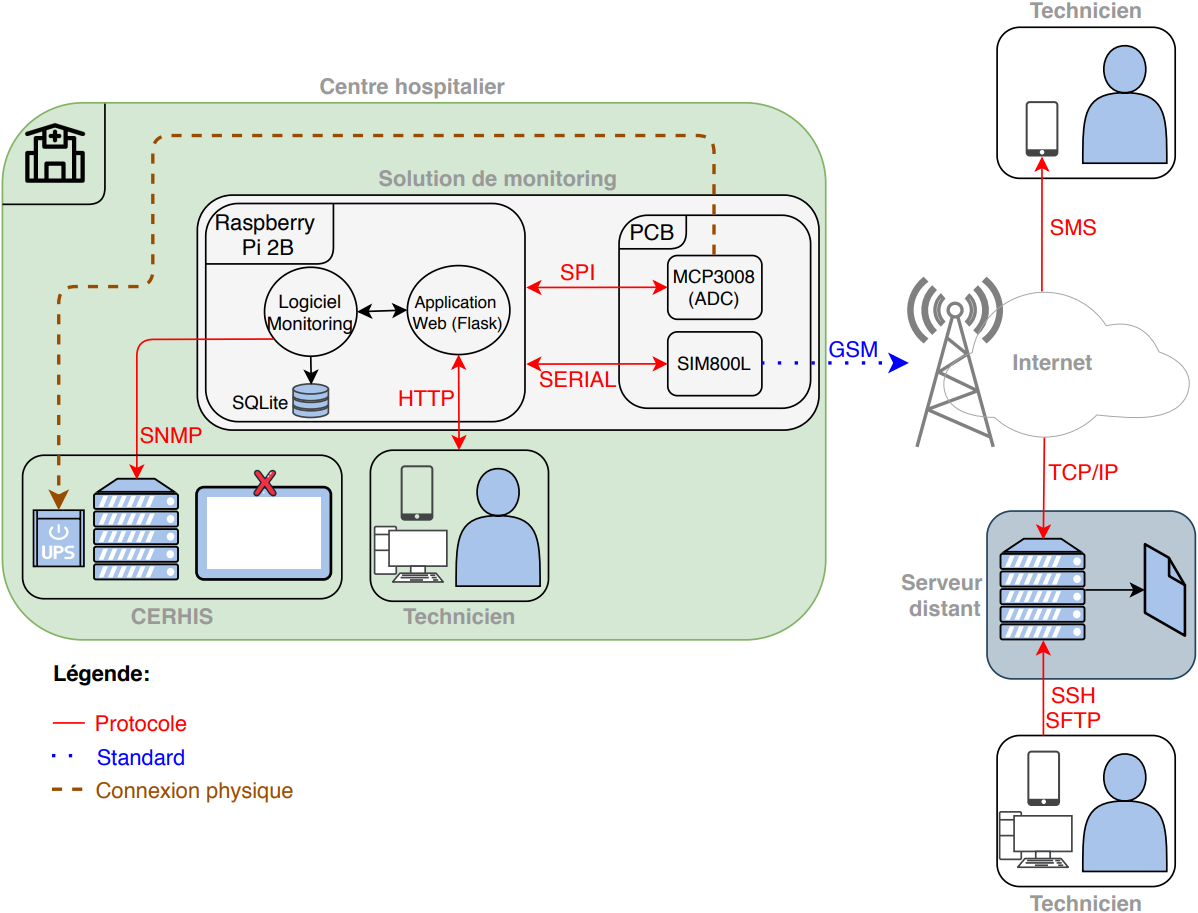
\includegraphics[width=\textwidth]{img/el_prototype/archi_prev.png}
  \caption{Architecture de la solution de monitoring développée lors de l'année académique 2018-2019}
  \label{fig:archi_prev}
\end{figure}



\noindent
Un Raspberry Pi 2B était utilisé pour tourner le logiciel de monitoring ainsi que l’interface web permettant la configuration de celui-ci. Un circuit imprimé (PCB) avait été réalisé dans le but de loger des composants électroniques différents tels que le module de communication GSM SIM800L et le convertisseur analogique numérique MCP3008. Ce même circuit imprimé s’insérait sur les ports GPIO du Raspberry Pi afin que ce dernier puisse interfacer avec les différents composants présents sur le PCB. Grâce au SIM800L, le réseau GSM d’un opérateur mobile local pouvait être utilisé pour envoyer des SMS vers un technicien, ou des informations quelques conques vers un serveur distant.  Dans ce premier essai, ce serveur était juste capable de recevoir les données envoyées par le prototype et de les stocker sur un fichier \textit{.txt}. Aucun traitement ou visualisation des données n’était offert aux techniciens. De plus, le monitoring des tablettes n'a pas pu être implémenté par manque de temps.

~

\noindent
De façon à alimenter le dispositif, un système d’alimentation mixte avait été mis en place. Comme le montre la figure \ref{fig:power_source}, ce système était basé sur une batterie acide-plomb de 12V, un régulateur de charge permettant de recharger la batterie et un convertisseur step-down transformant la tension de 12 à 5 volts.

~

\begin{figure}[ht!]
  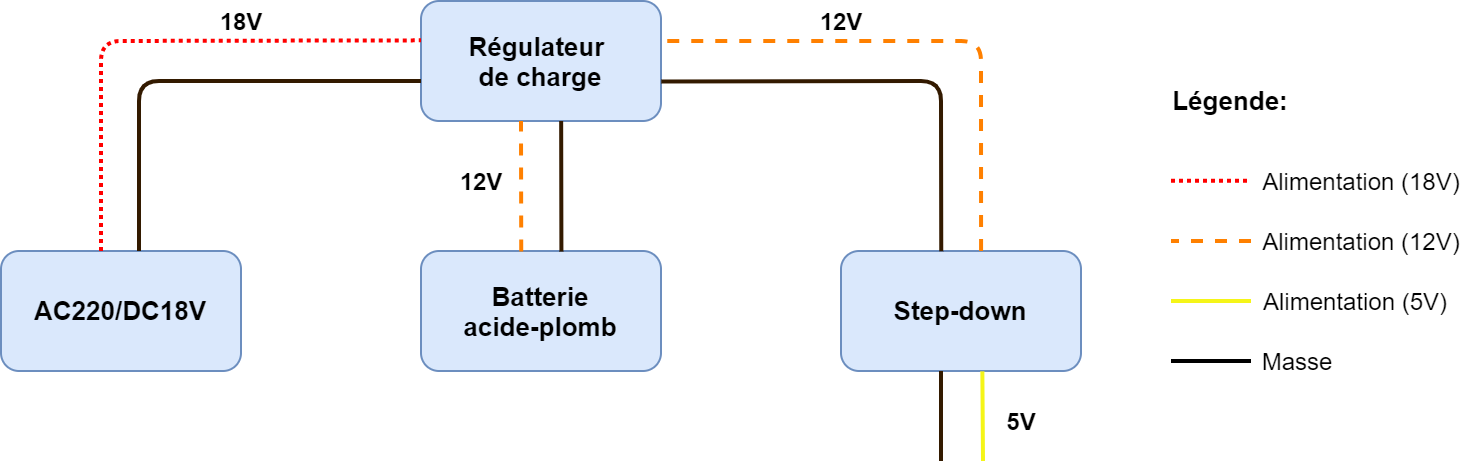
\includegraphics[width=\textwidth]{img/el_prototype/power_source.png}
  \caption{Système d'alimentation de la solution de monitoring développée lors de l'année académique 2018-2019}
  \label{fig:power_source}
\end{figure}

~

\noindent
Ce prototype a été testé pendant plusieurs semaines\footnote{entre le 14 mars et le 10 avril 2019} à Goma par un étudiant de l’ISIG\footnote{Institut supérieur d'informatique et de gestion de Goma}. Lors de cette période de tests, plusieurs problèmes ont été identifiés. Ils seront présentés dans la section suivante.

\subsection{Problèmes détectés}

Plusieurs protocoles de tests avaient été mis en place l’année dernière dans le but d'évaluer ce premier dispositif. Les soucis qui ont été trouvés lors de ces tests peuvent être classés selon trois grandes catégories : communication, alimentation et température. Tous les problèmes sont documentés ci-dessous.

\begin{itemize}
  \item \textbf{Communication :}
  \begin{itemize}
    \item Corruption de certaines données échangées entre le SIM800L et le Raspberry Pi. Des bits semblaient être modifiés lors de la transmission des messages entre les deux composants. Cela provoquait une perte d’informations. De plus, cela rendait plus difficile l'utilisation du SIM800L, car ce dernier n’était pas capable de traiter toutes les commandes qui lui étaient envoyées.

    \item Implémenter toutes les fonctionnalités de communication requises avec le SIM800L était très laborieux. En effet, ce module peut être vu comme un automate fini déterministe. Des commandes AT sont utilisées pour contrôler le module, c’est-à-dire qu'elles sont employées pour changer l’état de celui-ci. Une succession correcte de multiples commandes est nécessaire afin d'accomplir une simple tâche telle que l'envoi d'un SMS. Ceci rendait le procès d’implémentation assez long, en particulier l’implémentation de la gestion des erreurs. Le problème mentionné ci-dessus a encore plus aggravé la complexité de la manipulation de ce module.
  \end{itemize}

  \item \textbf{Alimentation :}
  \begin{itemize}
    \item Le régulateur de charge initialement utilisé est tombé en panne lors de la réalisation des tests. Un simple remplacement de cette pièce semble avoir résolu le problème.

    \item Le transformateur step-down est tombé en panne lors des tests. Malheureusement, aucun remplacement pour cette pièce a été trouvé à Goma. Ce souci est possiblement lié au problème de température qui sera présenté ci-dessous. Cependant, n’ayant pas assez d’information pour prouver l‘existence d'un lien de causalité, chaque problème doit être considéré séparément.
  \end{itemize}

  \item \textbf{Température :}
  \begin{itemize}
    \item D’après les personnes en charge de tester le prototype, celui-ci semblait atteindre de hautes températures. Des températures élevées peuvent avoir un impact considérable sur la durée de vie des différents composants électroniques.
  \end{itemize}
\end{itemize}

% \subsubsection{Influence sur le nouveau prototype}

\section{Nouveau Prototype}

\subsection{Solutions considérées}
\subsection{Thingstream}
\subsection{Résultat}
\subsection{Tests réalisés}
